\documentclass[12pt,portrait]{article}
\usepackage[round]{natbib}
\usepackage{times,amsmath,amsfonts}
\usepackage[dvips]{graphicx,graphics}


\usepackage{multirow}
\usepackage{amsfonts,amsmath,amssymb}
\usepackage{url}
\usepackage{hyperref}
\hypersetup{colorlinks,%
citecolor=red,%
filecolor=black,%
linkcolor=red,%
urlcolor=red,%
pdftex}

%\newcommand{\blue}[1]{{\color{blue} #1}}
%\newcommand{\green}[1]{{\color{green} #1}}
%\newcommand{\red}[1]{{\color{red} #1}}

\newtheorem{theorem}{Theorem}
\newtheorem{definition}{Definition}
\newtheorem{example}{Example}

\newcommand{\bq}{\begin{eqnarray*}}
\newcommand{\eq}{\end{eqnarray*}}
\newcommand{\bqn}{\begin{eqnarray}}
\newcommand{\eqn}{\end{eqnarray}}

\usepackage{wrapfig}
\usepackage{epsfig,psfrag}

\begin{document}
%\pagenumbering{arabic}
\pagenumbering{gobble}

\title{How to Write Papers
}
\author{Moo K. Chung\\
University of Wisconsin-Madison\\
\quad \tt{mkchung@wisc.edu}}
\maketitle 

\begin{abstract}
This short article explains how to write papers (conference, journal and final project report) that is more than 10 pages excluding figures, tables and references. Including all, it should be about 15 pages or more. The LeTex package for this article itself can be used to write a paper.  If you are not proficient in using LeTex, there is no need to use latex and MS-WORD or any other paper writing tool can be used. The abstract summarizes your research or survey and its outcomes without technical details. 
\end{abstract}

\section{Introduction}


The introduction of the paper expands the abstract and list main contributions of the paper with respect to existing literature. This is where you do literature review explaining what similar works have been done by others. With that list of literature, you contrast your main contribution of the research. It is expected you list reasonable number of previous papers. Try to add at least 10-20 references and explain what is new or different about your method with respect to existing methods in literature. You need detailed review discussing cons and pros of existing methods against your method. Also you need to able to spell out at least 2-3 major contributions or key points of the research.



\section{Methods}

{\bf Description of data:} The method section explains in detail what the data set is. Enough detailed explanation about data and preprocessing on the data is a must. For instance, you need to explain about what scanner was used and what is the image resolution and image acquisition parameters are. If you have your own data, you can use it after consultation with the instructor.\\


{\bf Methods:}  Then you describe in great detail what methods you used in analyzing the data.  It is expected you will be using one of the methods we studied in the class. \\

{\bf Validation \& comparisons:} This is where you justify your method using validation and comparisons against existing baseline methods using the real data and simulated data. Validate your methods with the ground truth data. Sufficient enough details should be added for any reader to duplicate the proposed method. Compare your methods to existing baseline methods. Demonstrate why your method is better than other methods. Also need to discuss how you will compare your method to existing methods. However, if your method is the first method to do something in the field, often you don't need comparisons since there are no existing method to compare. This is not likely unless you perform a ground breaking new innovative research. 


\section{Results}
Results are often given in tables (Table \ref{tab:gm_nodiff}), figures (Figure \ref{fig:meantop}), plots and quantitative numbers. Simply displaying pretty figures is not results. Must have quantitative numbers to demonstrate your method. Also you need to provide an interpretation of the results. Must also provide interpretation of the results. 


\begin{table}[t] 
\caption{Sample table summarizing the performance of the proposed topological loss $\mathcal{L}_{top}$ over other baseline methods. Generated by a former student who took the class \citep{song.2020.arXiv}.}
\label{tab:gm_nodiff}
\centering
\resizebox{\textwidth}{!}{
\begin{tabular}{ccc|ccccc}
    $d$ & $c$ & $p$ & GA & SM & RRWM & IPFP & $\mathcal{L}_{top}$ \\
    \hline 
    \multirow{6}{*}{12 vs. 12} & \multirow{2}{*}{2 vs. 2}   & 0.6 & $ 0.49 \pm 0.27 $ & $ 0.46 \pm 0.30 $ & $ 0.51 \pm 0.30 $ & $ 0.47 \pm 0.28 $ & $ 0.53 \pm 0.29 $ \\
                                 &                            & 0.8 & $ 0.45 \pm 0.25 $ & $ 0.47 \pm 0.31 $ & $ 0.56 \pm 0.29 $ & $ 0.47 \pm 0.30 $ & $ 0.50 \pm 0.30 $ \\
                                 & \multirow{2}{*}{3 vs. 3}   & 0.6 & $ 0.45 \pm 0.32 $ & $ 0.44 \pm 0.26 $ & $ 0.47 \pm 0.27 $ & $ 0.51 \pm 0.30 $ & $ 0.46 \pm 0.31 $ \\
                                 &                            & 0.8 & $ 0.54 \pm 0.31 $ & $ 0.51 \pm 0.27 $ & $ 0.51 \pm 0.29 $ & $ 0.52 \pm 0.29 $ & $ 0.51 \pm 0.30 $ \\
                                 & \multirow{2}{*}{6 vs. 6} & 0.6 & $ 0.57 \pm 0.30 $ & $ 0.51 \pm 0.28 $ & $ 0.56 \pm 0.29 $ & $ 0.45 \pm 0.26 $ & $ 0.58 \pm 0.29 $ \\
                                 &                            & 0.8 & $ 0.55 \pm 0.29 $ & $ 0.48 \pm 0.26 $ & $ 0.52 \pm 0.27 $ & $ 0.54 \pm 0.30 $ & $ 0.49 \pm 0.27 $ \\

    \hline \hline
    
    \multirow{6}{*}{18 vs. 18} & \multirow{2}{*}{2 vs. 2}   & 0.6 & $ 0.48 \pm 0.26 $ & $ 0.49 \pm 0.32 $ & $ 0.54 \pm 0.29 $ & $ 0.47 \pm 0.30 $ & $ 0.54 \pm 0.31 $ \\
                                 &                            & 0.8 & $ 0.52 \pm 0.28 $ & $ 0.50 \pm 0.28 $ & $ 0.46 \pm 0.30 $ & $ 0.52 \pm 0.25 $ & $ 0.50 \pm 0.26 $ \\
                                 & \multirow{2}{*}{3 vs. 3}   & 0.6 & $ 0.49 \pm 0.28 $ & $ 0.58 \pm 0.31 $ & $ 0.43 \pm 0.28 $ & $ 0.51 \pm 0.27 $ & $ 0.53 \pm 0.30 $ \\
                                 &                            & 0.8 & $ 0.46 \pm 0.30 $ & $ 0.51 \pm 0.27 $ & $ 0.52 \pm 0.33 $ & $ 0.45 \pm 0.29 $ & $ 0.53 \pm 0.27 $ \\
                                 & \multirow{2}{*}{6 vs. 6} & 0.6 & $ 0.53 \pm 0.28 $ & $ 0.48 \pm 0.30 $ & $ 0.51 \pm 0.30 $ & $ 0.45 \pm 0.29 $ & $ 0.44 \pm 0.33 $ \\
                                 &                            & 0.8 & $ 0.54 \pm 0.27 $ & $ 0.52 \pm 0.30 $ & $ 0.48 \pm 0.26 $ & $ 0.52 \pm 0.31 $ & $ 0.43 \pm 0.30 $ \\

    \hline \hline
    
    \multirow{6}{*}{24 vs. 24} & \multirow{2}{*}{2 vs. 2}   & 0.6 & $ 0.52 \pm 0.28 $ & $ 0.49 \pm 0.30 $ & $ 0.50 \pm 0.30 $ & $ 0.48 \pm 0.28 $ & $ 0.55 \pm 0.26 $ \\
                                 &                            & 0.8 & $ 0.53 \pm 0.27 $ & $ 0.56 \pm 0.30 $ & $ 0.51 \pm 0.30 $ & $ 0.56 \pm 0.32 $ & $ 0.52 \pm 0.30 $ \\
                                 & \multirow{2}{*}{3 vs. 3}   & 0.6 & $ 0.48 \pm 0.29 $ & $ 0.54 \pm 0.27 $ & $ 0.49 \pm 0.26 $ & $ 0.49 \pm 0.30 $ & $ 0.52 \pm 0.30 $ \\
                                 &                            & 0.8 & $ 0.55 \pm 0.29 $ & $ 0.49 \pm 0.27 $ & $ 0.52 \pm 0.28 $ & $ 0.49 \pm 0.30 $ & $ 0.47 \pm 0.26 $ \\
                                 & \multirow{2}{*}{6 vs. 6} & 0.6 & $ 0.47 \pm 0.30 $ & $ 0.45 \pm 0.31 $ & $ 0.51 \pm 0.29 $ & $ 0.56 \pm 0.28 $ & $ 0.49 \pm 0.29 $ \\
                                 &                            & 0.8 & $ 0.51 \pm 0.30 $ & $ 0.47 \pm 0.28 $ & $ 0.54 \pm 0.28 $ & $ 0.56 \pm 0.31 $ & $ 0.51 \pm 0.31 $ \\

    \hline
    
\end{tabular}}
\end{table}


\begin{figure}
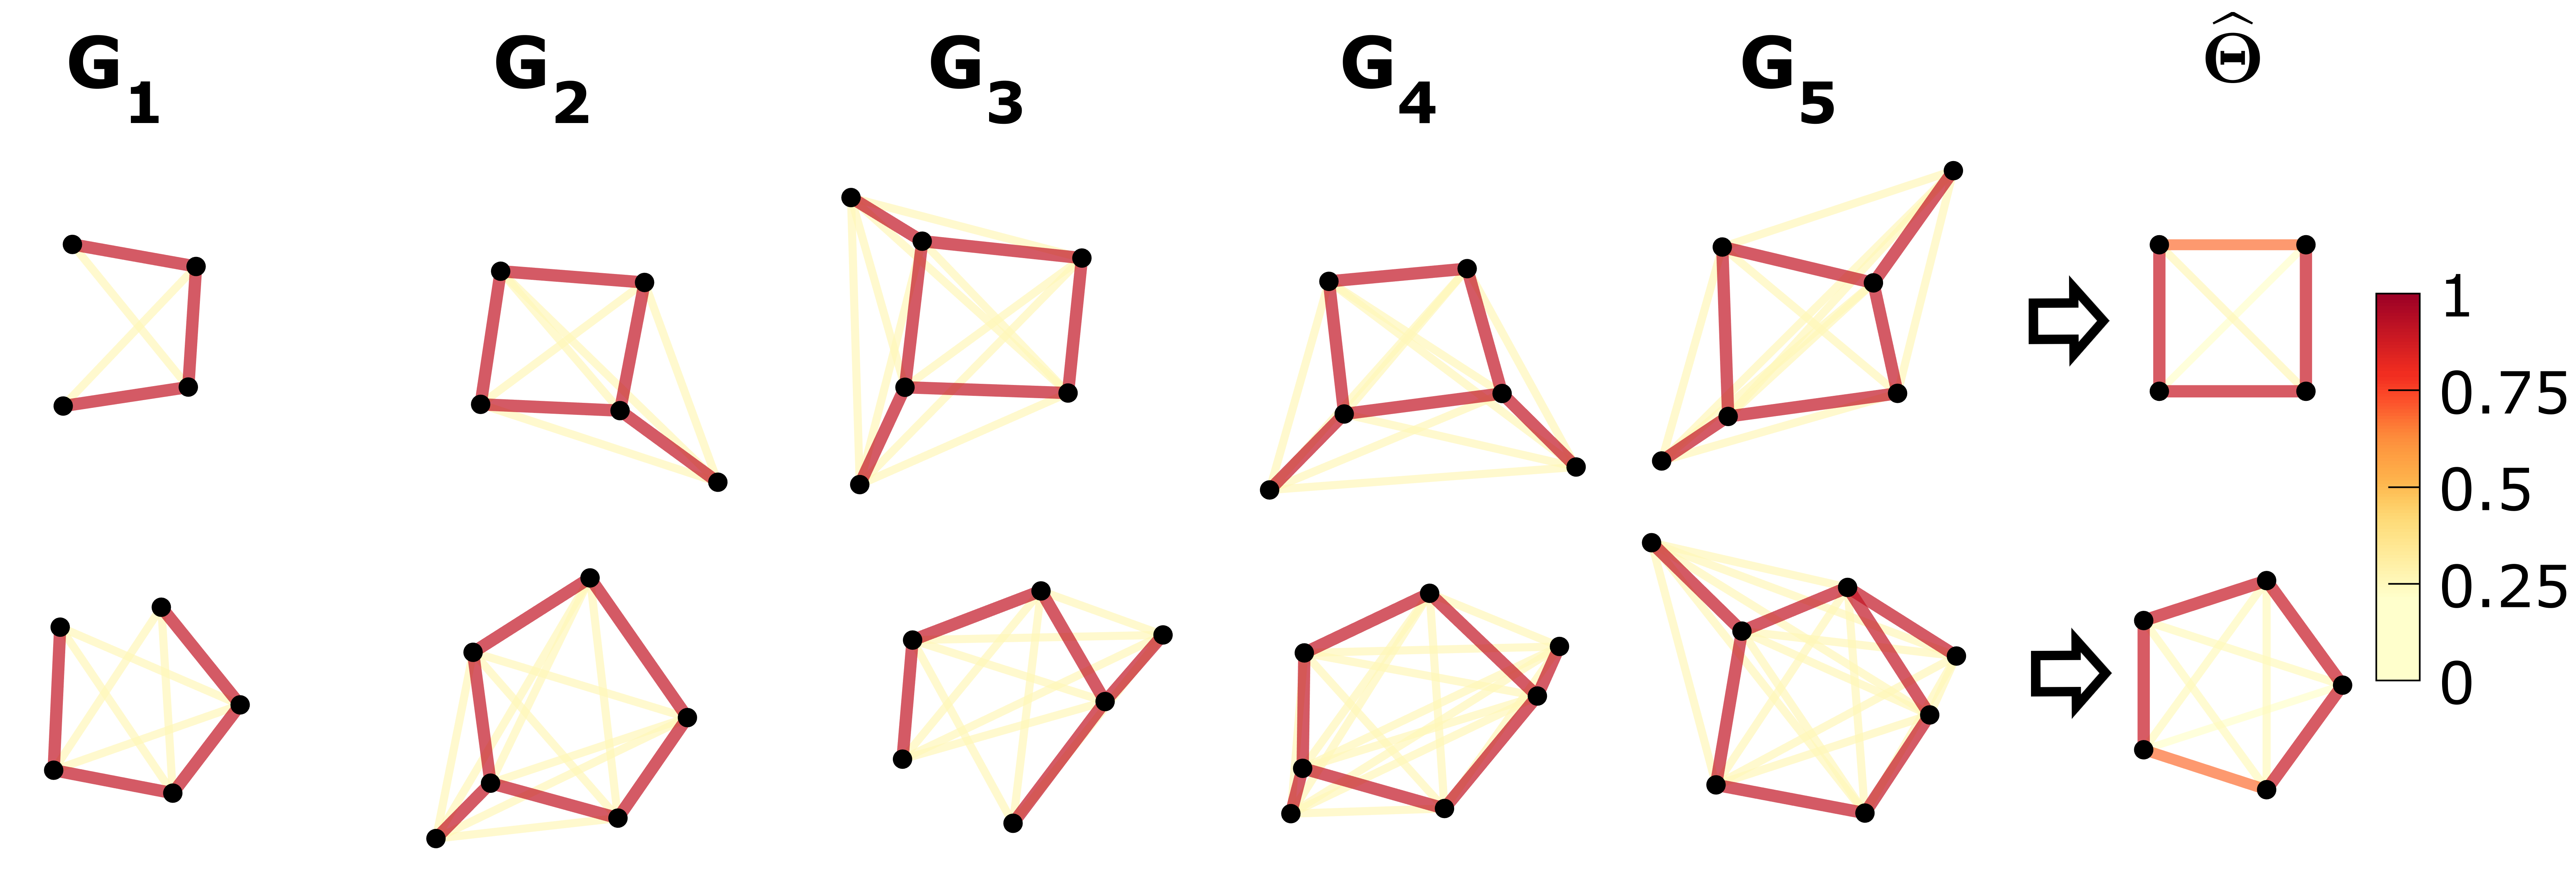
\includegraphics[width=1\linewidth]{toy_meantop.png}
\centering
\caption{\small Figure illustrating how to average graphs of different sizes and topology using persistent homology. Generated by a former student who took the class \citep{song.2020.arXiv}.}
\label{fig:meantop}
%\vspace{-0.5cm}
\end{figure}







\section{Discussion}
Discuss the limitation of your method. Discuss what you could have done better for future studies. Discuss what you did not do that you could have done. Often putting incomplete results into discussion is a good idea. You can also provide   an alternate strategy in case the proposed method did not perform well.


\section{Conclusion}
Concluding remarks. State what conclusion you obtained from the research. 

\section{References}
Provide minimum 10-20 relevant references to your method. The journal paper is cited as \citet{chung.2001.NI} while conference paper is cited as \citet{chung.2003.CVPR}. Books are cited as \citet{chung.2012.CNA}. See reference below to see how these citations are listed. You should reference more than 10 papers for research paper. For survey and literature review paper, you should cite more than 20 papers. 

\bibliographystyle{plainnat}
\bibliography{reference.2021.01.21}

\newpage 
\section{Evaluation Criteria}

The final research project report will be evaluated based on the following criteria, with each component contributing to the overall score:

\begin{itemize}
    \item \textbf{Structure and Organization, Literature  (25\%)}: The report should follow a logical structure, including a clear introduction, methodology, results, discussion, and conclusion. Sections should be well-organized, with coherent transitions between topics.  The report should demonstrate a thorough understanding of relevant literature. Proper citations should be included, and the background section should provide sufficient context for the research problem.
    

\item \textbf{Methods and Validations (25\%)}: The proposed methods must be clearly described with appropriate mathematical formulations, algorithmic descriptions, and implementation details. Students must demonstrate a strong understanding of the selected techniques, including their theoretical foundations, assumptions, and potential limitations. Justifications for the chosen approaches should be provided, ensuring that they are methodologically sound and logically structured for practical application in medical image analysis. 

The report must also include a rigorous validation of the proposed methodology using either statistical simulations covered in class or well-known baseline validation datasets. This may involve quantitative evaluation through appropriate performance metrics, qualitative assessments via visualizations, or comparisons with established benchmarks. Experimental results should be reproducible and well-documented to ensure independent verification. Any limitations in the validation process should be acknowledged, with suggestions for potential improvements. The discussion should critically analyze the strengths and weaknesses of the approach, demonstrating a deep understanding of its applicability in medical image analysis.


\item \textbf{Relevance to Course Materials (25\%)}: The selected methods (equations, formulations, algorithms, etc.) must be \underline{directly} related to the topics covered in class. Only methods that closely align with the course content will be evaluated; any methods outside the scope of the course will \underline{not} be considered. This requirement ensures that students fully engage with the core concepts presented in lectures and discussions, thus deepening their grasp of the material. By focusing on class-based methods, students can effectively demonstrate their mastery of key theoretical and practical components, while also fostering critical thinking skills as they apply these techniques to real-world medical image analysis. Additionally, maintaining strict relevance to course materials promotes fairness in assessment, as all students are evaluated based on the same foundational knowledge. 


{\it Example.} If you are implementing a diffusion-based learning method that was not covered in class, you must connect it to the diffusion equation discussed in class and clearly establish the detailed relationship between your approach and the covered diffusion equations. Failure to make this connection explicit will result in a loss of credit.




\item \textbf{Technical Writing, Results, and Conclusion (25\%)}: The report should be written in \underline{clear, precise}, and grammatically acceptable English. Technical terms should be properly defined, and explanations should be accessible. The results should be presented with clarity, incorporating tables, figures, or graphs where appropriate. Additionally, the report should provide a concise summary of findings, discuss their implications, and suggest potential future directions for research in medical image analysis.
    
Each criterion will be graded individually, and the final score will be determined by summing the weighted contributions of each category. Proper formatting, adherence to guidelines, and originality will also be considered in the final evaluation.


\item \textbf{Due Date}: The report is due by 9:30 AM on the last day of class. Students must submit the final project report in PDF format, along with all relevant materials demonstrating proof of effort, in a compressed (zipped) file to {\tt mkchung@wisc.edu}. The email submission will serve as the official record, as it carries an official school timestamp, and it will be the only accepted method of submission. A receipt of acceptance will be issued upon successful submission. Late submissions will incur a penalty of a \underline{1\% deduction} from the final score per hour past the deadline.

\item \textbf{Bonus}: Students who deliver a 30-minute oral presentation of their research project will receive a 1\%--10\% bonus, along with constructive feedback from the instructor and classmates to improve the final report. 


\item \textbf{Flagrism}: Students are expected to complete their work independently, without seeking or receiving help from any external person other than the instructor. All content, including code, text, tables, figures, and analyses, must be the student's own original effort. The use of ChatGPT (the only form of AI allowed in this class) is permitted but must be acknowledged. Students should note that any \underline{incorrect} information generated by ChatGPT and used in the report will be penalized. Using unauthorized assistance or plagiarizing from published materials, online resources, or other students is a serious violation of academic integrity. If a student is found to have engaged in such misconduct, they will forfeit any course credit and may face additional disciplinary actions in accordance with UW–Madison policies.



\end{document}
